% !TeX root =../../main.tex

\chapter{The FOT Fuzzing Framework} \label{ch:fot}


\section{Introduction}

Greybox fuzzing has become one of the most effective approaches~to detect vulnerabilities in a program under test (PUT).
Compared~with whitebox and blackbox fuzzing, greybox fuzzing strikes a balance~between execution speed and effectiveness.
The past years have witnessed a number of greybox fuzzing frameworks, e.g., {\AFL}~\cite{afl}, libFuzzer~\cite{libfuzzer}, and honggfuzz~\cite{honggfuzz}, followed by  various fuzzing extensions \cite{Bohme:2016:CGF,LiCMLLT17,Bohme:2017:DGF,CollAFL,nezha} to enhance their effectiveness and/or efficiency.


However, there lacks a fuzzing framework to easily reuse, integrate and compare different fuzzing techniques and~experiment with new ideas.
Take {\AFL} as an example, it is implemented~all in one file with around 8K LOC, which contains more than 100 global variables.
Hence, the implementation of a single feature often involves modifications in multiple places.
In short, {\AFL} is compact but also highly coupled because {\AFL} is designed to \textit{require essentially no configuration}~\cite{afl}.
In fact, most of the existing fuzzers are designed for easy deployment and usage, but not easy extension.
Therefore, it is desirable to have a fuzzing framework that allows easy \emph{configuration} and \emph{extension} for new features.





To this end, we propose our fuzzing framework, namely Fuzzing~Orchestration Toolkit  ({\FOT}). {\FOT} is designed to hold three properties.

\begin{enumerate}[(1)]


\item  \textbf{Versatility.}
{\FOT} provides a fuzzing ecosystem, including a set of static~and dynamic analyses used to aid the fuzzing process.


\item \textbf{Configurability.}
{\FOT} provides a set of configurable options.
Users can easily tweak the parameters of the fuzzer to improve the fuzzing effectiveness with their experience.

\item \textbf{Extensibility.}
{\FOT} is designed to be of high coherence and low coupling. Specially, the implementation mainly consists of two parts: the library containing general fuzzing utilities and miscellaneous tools on top of it. Therefore, apart from the default fuzzer provided by {\FOT}, developers can write their own fuzzers with modest effort based on the library.
\end{enumerate}







 

\section{Architecture Design}\label{sec:details}

In this section, we describe the design of {\FOT} framework.
Interested readers can refer to {FOT}'s project site for more details:
\url{https://sites.google.com/view/fot-the-fuzzer}.


\begin{figure}[t]
	\centering
	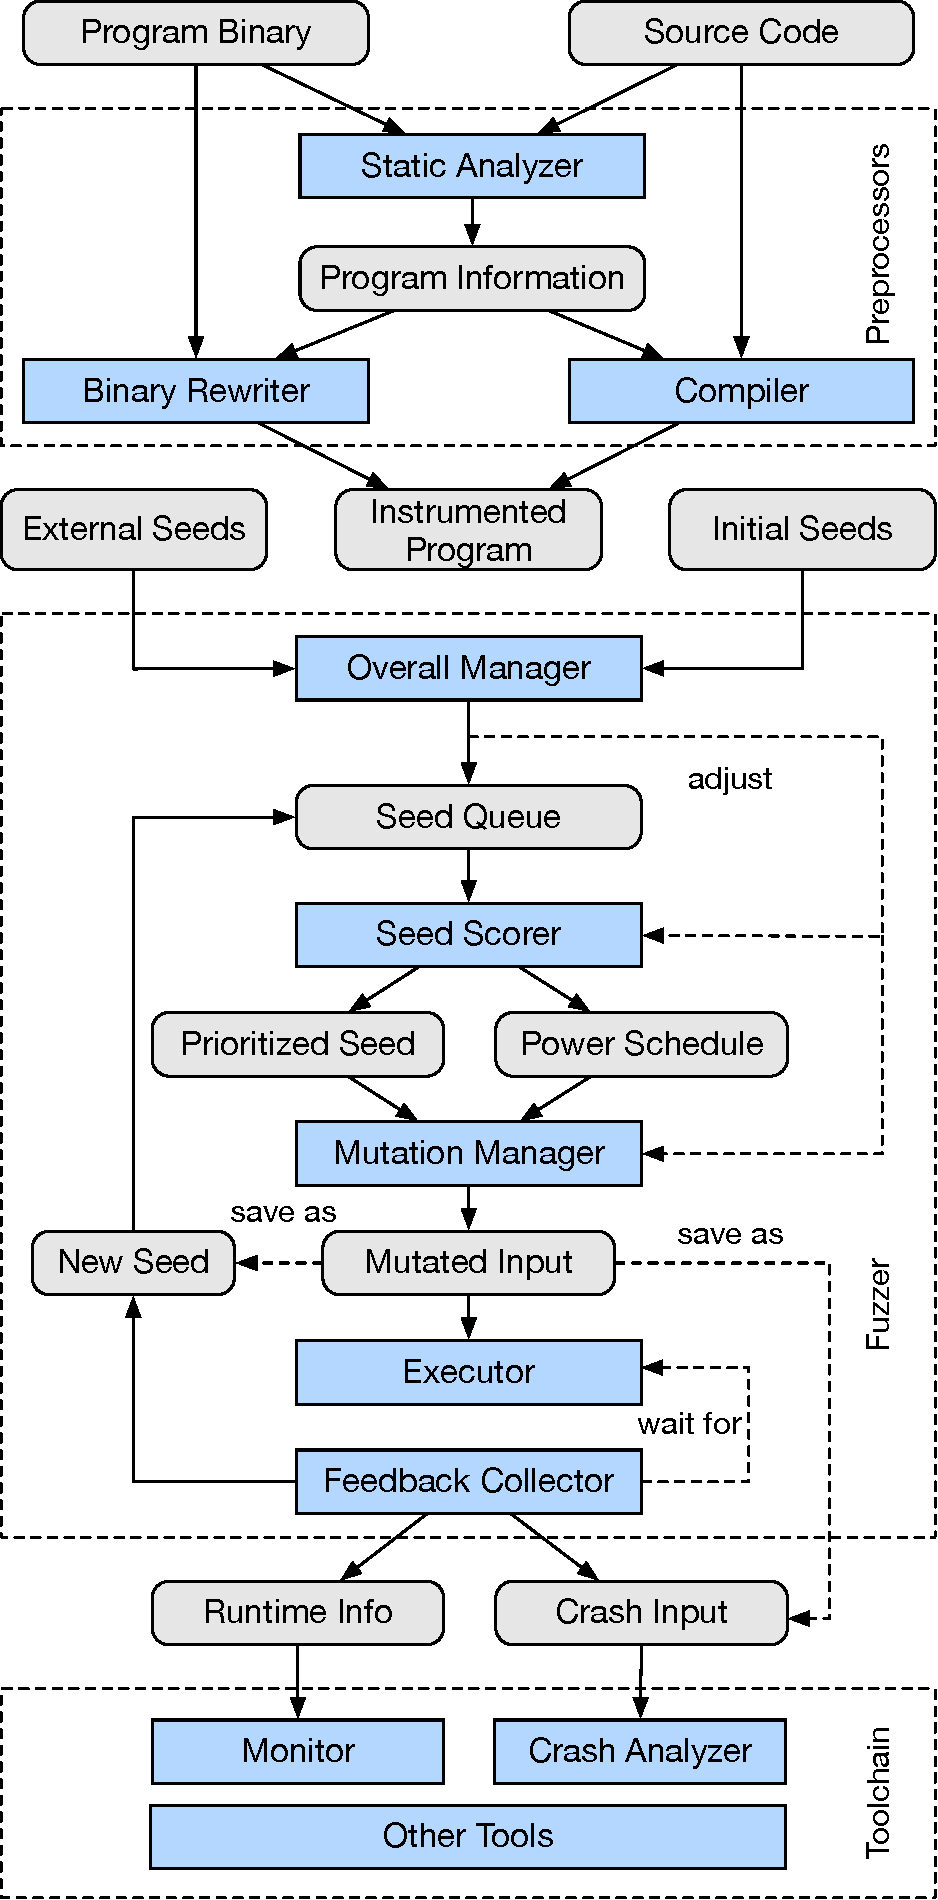
\includegraphics[width=0.46\textwidth]{res/fot/FOT_overview}
	\vspace{-5pt}
	\caption{Overview of the {\FOT} Fuzzing Framework}
	\label{fig:fot_workflow}
\end{figure}




Figure~\ref{fig:fot_workflow} depicts the overview of {\FOT}.
It consists of three parts, namely the \emph{preprocessor}, the \emph{fuzzer}, and the \emph{complementary toolchain}.
Components of the framework are represented with \emph{blue} rectangles. All these components are \textit{configurable} and \textit{extensible}.


\subsection{Preprocessor}
This part contains various tools for collecting static information and instrumentation with the PUT.


\subsubsection{Static Analyzer}\label{sec:static_analysis}
This includes various tools to extract semantic understandings from the PUT.
For example, we have tools to generate the control flow graph, call graph or statically collected vulnerability information and convert them into suitable representations that can later be instrumented into the PUT and utilized during the fuzzing process.
This part is \textit{configurable} to generate different levels of static information. It is \textit{extensible} as developers are allowed to add new types of static analysis as long as the generated result follows the specified format.


\subsubsection{Instrumentor}
The \emph{binary rewriter} and the \emph{compiler} instrument additional static information generated by the static analyzer into the PUT so that the fuzzer can collect feedback from the latter during execution.
{\FOT} supports Dyninst~\cite{dyninst} based instrumentation when only binary is provided, and LLVM based instrumentation when the source code is available.
This part is \textit{configurable} as the users can choose to either instrument at source code level or at binary level.
It is \textit{extensible} since developers can use other tools such as Intel Pin~\cite{pin} for instrumentation as long as the instrumented code can embed the static information and follow the regulations to provide feedback for the fuzzer.

\subsection{Fuzzer}
This part explains {\FOT}'s the main fuzzing process. 
It is essentially a loop that continuously selects seeds from the queue, applies mutations to the selected seeds, executes the PUT against mutated inputs, and collects feedback for the next iteration.

\subsubsection{Overall Manager}
As {\FOT} is designed to support multi-threaded parallel fuzzing, it contains an overall manager for fuzzing, managing the workload of each worker thread.
Particularly, it can listen to a special directory to actively import seed inputs from external sources such as symbolic executors like KLEE~\cite{klee} or mutation generators like Radamsa~\cite{radamsa}.
This part is \textit{configurable} as the users can choose different strategies for the overall management.
It is \textit{extensible} as it can interoperate with other seed generation tools.


\subsubsection{Seed Scorer}
The seed scorer is in charge of selecting a seed from the queue for mutation (seed prioritization) and determining how many new inputs should be generated based on the selected seed (power scheduling).
This part is \textit{configurable} as the users can select from several built-in scoring strategies to evaluate seeds.
It is \textit{extensible} as the users can implement their own strategies with the interfaces provided in {\FOT}.


\subsubsection{Mutation Manager}
The mutation manager is in charge of incorporating different mutators.
It can mutate the seeds in a pure random manner or according to predefined specifications.
This part is \textit{configurable} as {\FOT} provides various mutators for the users to choose from.
It is \textit{extensible} as the developers can implement their own mutators with the provided library.

\subsubsection{Executor}
The executor drives the execution of the PUT.
This part is \textit{configurable} as the default executor in {\FOT} allows users to choose whether or not to use forkserver~\cite{afl} during fuzzing.
It is \textit{extensible} as the developers can extend the executor for different scenarios.
For example, they may add a secondary executor to execute another PUT to perform differential testing.

\subsubsection{Feedback Collector}
The feedback collector collects the feedback emitted by the PUT.
The exact feedback often corresponds to the instrumented information.
This part is \textit{configurable} as the users are allowed to select from the default feedback options provided by {\FOT}.
For now, the feedback can be at basic-block level (like {\AFL}) or function level.
It is \textit{extensible} as the users can specify their customized types of feedback for collection.

\subsection{Complementary Toolchain}
{\FOT} additionally contains various tools helping to make the framework \textit{versatile}.
For instance, we implemented a web-based frontend user interface to monitor the fuzzing results.
It provides fruitful information to make the fuzzing process more transparent.
We also implemented a crash analyzer to analyze the detected crashes and generate reports automatically.
This reduces the manual efforts of crash triaging.
Last but not the least, several other tools have been developed with different purposes to complement the fuzzer.


















\begin{comment}
\subsection{Trace Update and Synchronization}\label{sec:trace_sync}
One of {\FOT}'s key features is the trace synchronization between fuzzing workers. In general we followed {\AFL}'s practice (c.f. Listing~\ref{lst:afl-inst}) to instrument the target program; but we made a slight change to the instrumentation runtime to make the target binaries able to distinguish different shared memory arenas and the file descriptors used for ``forkserver'' allocated/specified by different fuzzing workers~\footnote{The ``forkserver'' hacking by {\AFL} is explained at \url{https://lcamtuf.blogspot.sg/2014/10/fuzzing-binaries-without-execve.html}.}. Each fuzzing worker allocates the shared memory and the instrumented binary writes to specific multiple 8-byte areas when the corresponding ``execution edges'' have been reached. By auditing the byte fingerprints, the fuzzer knows about the edges and their approximate hit counts within this run. This information sits between between ``branch coverage'' and ``path coverage''. By comparing the shared memory fingerprint with the local trace information (checking whether the active shared memory byte has been marked ``traced'' locally), the fuzzer gets the knowledge whether current running seed increases the coverage. Updating of the local trace is majorly a ``bitwise and'' where each byte of the local trace is initialized with all ones (i.e., 255).

The local trace is synchronized with the global trace state. There stands a tradeoff: if we use directly the global trace state, the synchronization will be too frequent and eventually decreases performance with the increase of more fuzzing workers; if the fuzzers are only aware of the local trace, it is no better than {\AFL}'s na\"ive approach that runs all instances separately. We thus choose to only apply the synchronization during the mutation of each test case in the queue, when customizable conditions are triggered (usually the conditions are about the executions and time since last synchronization).

The actual synchronization of the trace information still applies ``bitwise and'' on normal running traces~\footnote{In practice, we also synchronize the timeout traces and crash traces to avoid generating too many redundant ``abnormal'' test cases.} from local trace information to global state, and an instant copy in the other direction. This is far more efficient than {\AFL}'s synchronization by 1) importing seeds from other directories and 2) running all the test cases indistinguishably. Note that {\FOT}'s synchronization does not lose precisions compared to {\AFL}'s, where both ``bitwise and'' operations erase the exact hit count information.
\end{comment}




\begin{comment}
  \subsection{Mutation Strategy Adaption}\label{sec:mutation_ops}
 The selection of mutation operators during fuzzing on one test input is determined by two factors:
 \begin{enumerate}
 	\item The whitelist mutation operators used for the targeted binaries. Some mutation operators are only effective on certain programs, but is almost a waste of time for the other programs (for example, bitflip operations are quite expensive and rarely useful for text-based parser programs running against large files). This can be specified by the experienced {\FOT} users.
 	\item The one-time mutation operators for \emph{this fuzz}. This is automatically determined by the fuzzer according to statistics generated from the previous mutations and runs. It is calculated in an adaptive way and may finally help to determine the ``convergence'' of the test cases.
 \end{enumerate}

{\AFL} has limited configurations for what mutation operators can be used and frequently runs blindly on the mutations that do not fit well.
 \end{comment}





\begin{comment}
\subsection{Refinement on Variable Behaviors}\label{sec:entry_var_behavior}

Some programs have variable behaviors for the same input test, due to randomness, multi-threading, etc. {\AFL} handles this issue by running all the newly found interesting test cases multiple times (known as \emph{calibration}); whenever it finds that the shared memory information (the active bytes and their hit count) differs from the first run, it will give more chances to the running test entry, and then keeps track of the variable behavior rate. The problem is that it does not utilize the information further since variable behaviors may cause certain runs to exit normally at some time, however crash at other time, which is more serious. We separately track those test case and give even more chances for these seeds. Alternatively, we provide an intrinsic strategy to prioritize these cases and let those test cases to be more likely to run next time (by using the prioritization in section~\ref{sec:seed_priority}). On the other hand, {\AFL}'s tracing information for the variable behavior cases are imprecise since it only traces the last calibration shared memory; we refine this by (selective) ``bitwise or'' operations to the shared memory for subsequent procedures on the current seed.


 \subsection{Trimming on duplicated cases}
Due to the existence of the potential lag of the trace synchronization, there still exists test input that runs with the same running trace. In other cases, the test cases might not be in its ``simplest'' form: by removing some bytes, the input test case can still results in the same running trace. {\FOT}'s approach in handling this is to trim the calibrated test cases immediately before being parceled as the message and sent to the message queue buffer managed by the conductor. And the conductor maintains a checksum set of all the generated seed files. Therefore when the newly generated seed has the same checksum as one of the existing ones, this test case will be discarded.

Additionally, we provide an external minimizer program to prune the all the serialized test cases (which can be normal runs, timeout runs, or crashes); it is more aggressive than the embedded procedure in the fuzzer and aims to provide a minimized version of all the interesting test cases.
\end{comment}

 

\section{Implementation and Extensions}\label{sec:app}

We have implemented the {\FOT} framework and developed two extensions to {\FOT}.

\subsection{Implementation}

The {\FOT} project started from June, 2017 and has been actively developed by two researchers. It is implemented with 15000 lines of Rust for core fuzzing modules, together with 2600 lines of C/C++ for the preprocessor, 4800 lines of Java for structure-aware mutation, and 2400 lines of Python for complementary toolchain.





\subsection{Static Vulnerability Analysis Integration}\label{subsec:sva}



Greybox fuzzers are typically aware of quantitative changes of code coverage and use such feedback for keeping the \textit{interesting} seeds.
However, the performance of collecting code coverage feedback quantitatively is often not ideal, and greybox fuzzers also need to evaluate the code coverage qualitatively~\cite{Bohme:2016:CGF}.
One of the approaches to bring qualitative awareness about the covered code is to combine fuzzing with static vulnerability analysis, as mentioned in \S~\ref{sec:static_analysis}.

\begin{figure}[!t]
	\centering
	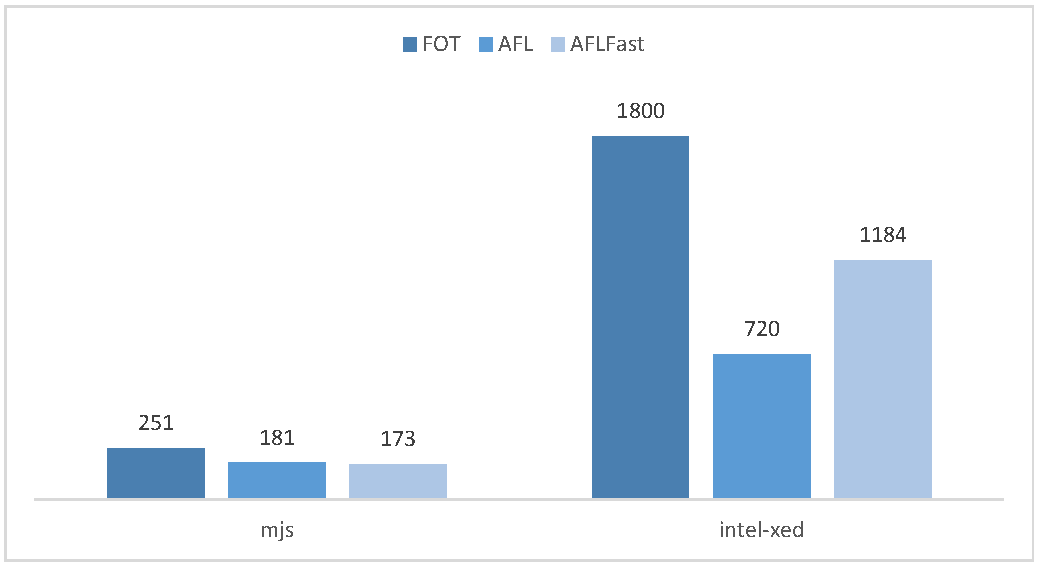
\includegraphics[width=0.4\textwidth]{res/fot/moo_result.pdf}
	\caption{Average Number of Unique Crashes Found in 24 Hours on \textit{mjs} and \textit{intel-xed}.}
	\label{fig:moo_result}
\end{figure}


Existing fuzzing works seldom use static analysis information to facilitate seed prioritization and power scheduling since existing fuzzing frameworks have little support for them.
In contrast, integration with vulnerability static analysis is trivial in \FOT: we used \emph{static analyzer} to calculate vulnerability metrics (e.g., calls~to unsafe functions and cyclomatic complexity) and customized \emph{seed scorer} to take them into account during fuzzing. This extension added about 330 lines of C++ and 190 lines of Rust code.

The workflow is as follows.
First, the static analyzer calculates vulnerability score for each function. Then we instrument the PUT to provide function level coverage information.
After detecting a seed that brings new coverage, the feedback collector will collect its function level coverage and map it with the static analysis result to get the function level vulnerability scores.
The seed scorer will then accumulate the function-level scores to form the execution trace level vulnerability scores for the exercised seeds.
Finally, the power schedule determined by the seed scorer prioritizes and allocates more powers to the seeds with higher vulnerability scores.



Figure~\ref{fig:moo_result} shows the average number of unique crashes detected on mjs and intel-xed of different fuzzers over 10 runs.
We can see that with the help of static vulnerability analysis, {\FOT} can detect more unique crashes in a limited time budget.
 

\subsection{Directed Greybox Fuzzing (DGF)}\label{subsec:dgf}

Guiding the greybox fuzzer towards certain predefined locations in the PUT can fit multiple scenarios such as patching testing, crash reproduction, and static analysis report verification~\cite{Bohme:2017:DGF}.






DGF requires the fuzzer to evaluate seeds according to their~distances towards target locations.
AFLGo~\cite{Bohme:2017:DGF} is a DGF based on {\AFL}. It applies a simulated-annealing-based power schedule for the seeds according to their distances from target locations.
However, building an effective directed fuzzer requires not only adjustments of \emph{power schedules} but also \emph{seed prioritization} and \emph{mutation strategies}.



DGF in {\FOT} is done by generating the static distances to the target locations with the help of \emph{static analyzer} and customized \emph{program instrumentation}, \emph{feedback collector}, \emph{seed scorer} as well as the \emph{mutation manager}. The implementation added about 240 lines of C++ and 510 lines of Rust code.

The workflow is as follows.
The preprocessor calculates the distances to target locations for each basic-block and function, and then instruments the basic-block level distance information during compilation.
During fuzzing, the fuzzer collects the distance information along the executed traces for the seeds.
The seed scoring module will prioritize the seeds closer to the targets and assign more powers to them. 
Moreover, the mutation manager will favor fine-grained mutations once the target function is reached.





%Table~\ref{tbl:cr_aflgo_binutils} compares the results of FOT with AFL and AFLGo on the c++filt tool in GNU Binutils (each experiment was conducted 20 times with 8 hours as the budget). {\utte} is the average time-to-exposure in seconds to trigger a vulnerability. We can see that {\dFOT} is able to decrease the exposure time greatly.
%
%\begin{table}[!t]
%	\small
%	\centering
%	\caption{Crash Reproduction in {\dFOT}, {\aflgo} and AFL Against Binutils (Taken from~\cite{hawkeye}).}
%	\label{tbl:cr_aflgo_binutils}
%	\vspace{-10pt}
%	\begin{tabular}{|c|c|r|r|c|}
%		\hline
%		\textbf{CVE-ID}   & \textbf{Tool}  & \textbf{Runs} & \utte (s)  & \textbf{Factor} \\ \hline\hline
%		\multirow{3}{*}{2016-4487}& FOT &   20    &   177   & -- \\ \cline{2-5} 
%		& AFLGo  &  20  & 390 & 2.20\\ \cline{2-5} 
%		&  AFL   &   20 & 630  &   3.56  \\ \hline
%\multirow{3}{*}{2016-4492} & FOT &     20      &                    477                                 &       --      \\ \cline{2-5} 
%		&   AFLGo  &     20   &  540  &                 1.21                                               \\ \cline{2-5} 
%		&    AFL   &     20   &                         960                            &                  2.01                                              \\ \hline
%		\multirow{3}{*}{2016-6131} & FOT &       9     &                     17314                                &                      --                                          \\ \cline{2-5} 
%		&   AFLGo  &                   6                                   &                      21180                               &                                1.22                                \\ \cline{2-5} 
%		& AFL   &                    2                                  &            26340                                         &             1.52                                                   \\ \hline
%		
%	\end{tabular}
%\end{table} 



%
 \subsection{New Vulnerabilities}



Till now, {\FOT} has been used to fuzz more than 100 projects.
Table~\ref{tbl:trophies} lists some of the 0-day vulnerabilities we found with {\FOT}. Among them, 6 CVEs have been assigned to Oniguruma (a widely used regular expression library used by PHP, Ruby, etc) and 9 CVEs have been assigned to Espruino (a Javascript engine for IoT devices). GNU diffutils, GNU bc and apcalc have been used for many years. Other projects such as radare2 (an open source reverse engineering framework) and libsass (the SASS library) have been fuzzed for multiple times by others.

\begin{table}[!t]
	\centering
	\caption{Selected Trophies and the Projects}
	\label{tbl:trophies}
	\vspace{-10pt}
	\begin{tabular}{|r|r|r|r|r|}
		\hline
		\multicolumn{1}{|c|}{\textbf{\begin{tabular}[c]{@{}c@{}}Project\\ Name\end{tabular}}} & \multicolumn{1}{c|}{\textbf{\begin{tabular}[c]{@{}c@{}}0-day\\ Bugs\end{tabular}}} & \multicolumn{1}{c|}{\textbf{\begin{tabular}[c]{@{}c@{}}Time Since\\ Release\end{tabular}}} & \multicolumn{1}{c|}{\textbf{\begin{tabular}[c]{@{}c@{}}GitHub\\ Stars\end{tabular}}} & \multicolumn{1}{c|}{\textbf{KLOC}} \\ \hline\hline
		mjs & 21 & 1y7m & 787 & 16.5 \\ \hline
		liblnk & 20 & 8y9m & 42 & 56.9 \\ \hline
		GNU bc & 18 & 26y8m & -- & 31.4 \\ \hline		
		radare2 & 10 & 9y4m & 7645 & 857.1 \\ \hline
		Espruino & 10 & 4y9m & 1395 & 1392.6 \\ \hline
		libsass & 10 & 6y5m & 3813 & 43.8 \\ \hline
		libpff & 7 & 3y8m & 85 & 137.7 \\ \hline
		Oniguruma & 6 & 5y8m & 556 & 119.1 \\ \hline		
		apcalc & 4 & 19y & -- & 98.7 \\ \hline
		FLIF & 3 & 2y9m & 2989 & 43.6 \\ \hline
		diffutils & 2 & 29y7m & -- & 147.4 \\
		\hline
	\end{tabular}
\end{table}

  

\section{Related Work}

In this section, we first compare FOT with other fuzzing frameworks, and then discuss its relationship to current fuzzing extensions.



\subsection{Comparisons to Other Fuzzing Frameworks}

Table~\ref{tbl:cmp_fuzz} compares {\FOT} with existing fuzzing frameworks with respect to 10 major features. As we can see, the existing fuzzing frameworks AFL, libFuzzer and honggfuzz lack features in different aspects, while {\FOT} integrates all of them. {\FOT} stands out in that it provides various configurations for advanced users; it is also highly modularized to be easily extended with other fuzzing techniques. Further more, {\FOT} also partially supports structure-aware mutations (by specifying semantic grammars) and interoperability with other seed generation tools such as symbolic executors (by monitoring and scheduling newly incoming seed input directory). 
\subsection{Relationship to Current Fuzzing Extensions}

Most current fuzzing techniques can be easily integrated into {\FOT} thanks to its highly-modularized design. In fact, these techniques can be applied with some extensions to the different components in Figure~\ref{fig:fot_workflow} and can be used together with the configuration interface. 

\begin{enumerate}[1)]
	\item AFLFast~\cite{Bohme:2016:CGF} can be implemented by applying a Markov Chain model based seed \emph{power scheduling} in the fuzzer. 
	\item AFLGo~\cite{Bohme:2017:DGF} can be implemented by a combination of \emph{static analyzer}, \emph{instrumentation} and \emph{power scheduling}.
	\item CollAFL~\cite{CollAFL} can be implemented by using a collision-resistant algorithm to increase the uniqueness of the path trace labeling during \emph{instrumentation}.
	\item Skyfire~\cite{junjie:2017sp:skyfire}, Radamsa~\cite{radamsa}, Csmith~\cite{csmith} can be used in the preprocessor to generate seeds for the \emph{external seeds} and a structure-aware mutator assigned by \emph{mutation manager}.
	\item Symbolic executors such as KLEE~\cite{klee} can be integrated in the Driller's~\cite{driller} style with the help of \emph{overall manager}.
\end{enumerate}

\begin{table}[t]
	\small
	\caption{Comparisons between Different Fuzzers (\Circle: not supported, \LEFTcircle: partially supported, \CIRCLE: fully supported)}
	\label{tbl:cmp_fuzz}
	\vspace{-10pt}
	\resizebox{.475\textwidth}{!}{
	\begin{tabular}{|l|c|c|c|c|}
		\hline
		\diagbox{\textbf{Features}}{\textbf{Framework}} & \textbf{AFL} & \textbf{libFuzzer} & \textbf{honggfuzz} & \textbf{FOT} \\ \hline\hline
		Binary-Fuzzing Support & \CIRCLE & \Circle & \CIRCLE & \CIRCLE \\ \hline
		Multi-threading Mode & \Circle & \CIRCLE  & \CIRCLE  & \CIRCLE  \\ \hline
		In-memory Fuzzing &\CIRCLE  & \CIRCLE &\CIRCLE  & \CIRCLE \\ \hline
		Advanced Configuration & \Circle  & \LEFTcircle  & \Circle  & \CIRCLE  \\ \hline
		Modularized Functionality & \Circle & \LEFTcircle & \Circle & \CIRCLE \\ \hline
		Structure-aware Mutation & \Circle  &\Circle & \Circle  & \LEFTcircle \\ \hline
		Interoperability & \Circle & \Circle & \Circle & \LEFTcircle \\
		\hline
		Toolchain Support &  \CIRCLE & \Circle  & \Circle  & \CIRCLE \\ \hline
		Precise Crash Analysis & \Circle  & \Circle  & \CIRCLE  & \CIRCLE  \\ \hline
		Runtime Visualization & \LEFTcircle & \Circle & \Circle & \CIRCLE \\ \hline
	\end{tabular}
}
\end{table}
 

\section{Conclusions}

We have proposed {\FOT}, a versatile, configurable, and extensible fuzzing framework to facilitate the reuse, integration, comparison and development of different fuzzing techniques. We briefly explained the workflow of {\FOT} and showed its applications in the aspects of static vulnerability analysis enhanced fuzzing and directed grey-box fuzzing. The experimental results have indicated that {\FOT} can be quite effective for different fuzzing scenarios.
 
\section*{Acknowledgment}
This work is supported by the National Research Foundation, Prime Ministers Office, Singapore under its National Cybersecurity R\&D Program (Award No. NRF2016NCR-NCR002-026) and administered by the National Cybersecurity R\&D Directorate; the research of Dr Xue is also supported by Chinese Academy of Sciences (CAS) Pioneer Hundred Talents Program of China.


